\documentclass{article}
\usepackage{tkz-graph}
\usetikzlibrary{arrows}
\usetikzlibrary{intersections, backgrounds}

\begin{document}

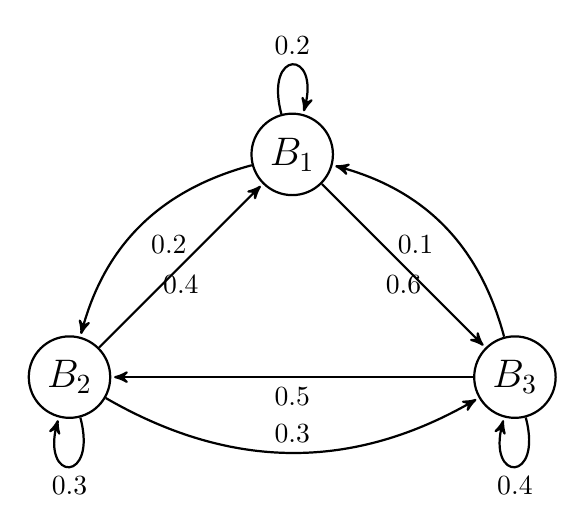
\begin{tikzpicture}[->,>=stealth',shorten >=1pt,auto,node distance=4cm,
                thick,main node/.style={circle,draw,font=\Large\bfseries}]

  \node[main node] (1) {$B_1$};
  \node[main node] (2) [below left of=1] {$B_2$};
  \node[main node] (3) [below right of=1] {$B_3$};

  \path
    (1) edge [loop above] node {0.2} (1)
        edge [bend right] node {0.2} (2)
        edge node [below]{0.6}(3)
    (2) edge node [below]{0.4} (1)
        edge [loop below] node {0.3} (2)
        edge [bend right] node {0.3} (3)
    (3) edge [bend right] node {0.1} (1)
        edge node[below] {0.5} (2)
        edge [loop below] node {0.4} (3);
\end{tikzpicture}


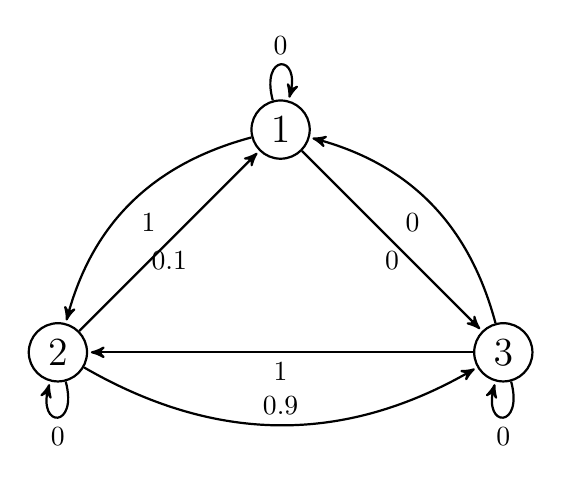
\begin{tikzpicture}[->,>=stealth',shorten >=1pt,auto,node distance=4cm,
                thick,main node/.style={circle,draw,font=\Large\bfseries}]

  \node[main node] (1) {$1$};
  \node[main node] (2) [below left of=1] {$2$};
  \node[main node] (3) [below right of=1] {$3$};

  \path
    (1) edge [loop above] node {0} (1)
        edge [bend right] node {1} (2)
        edge node [below]{0}(3)
    (2) edge node [below]{0.1} (1)
        edge [loop below] node {0} (2)
        edge [bend right] node {0.9} (3)
    (3) edge [bend right] node {0} (1)
        edge node[below] {1} (2)
        edge [loop below] node {0} (3);
\end{tikzpicture}



\end{document}
